\subsection{Day-ahead commitment under uncertainty}
\label{sec:res-dayahead}

\subsubsection{Commitment--operation pairing}
\label{sec:res-pairing}

Three commitments are compared on the case day and 20 operating days, each operated by IR-O* (with $\alpha$ re-tuned
for that commitment) and by JR-D: the single-event capability assessment (SE), the SE commitment scaled by the
back-tested factor $\theta^*=0.8$ (SE-$\theta$, a cautious conventional practice), and the coupled day-ahead commitment
(DA) (\tabref{tab:pairing}, \figref{fig:pairing}).

\begin{table}[!t]
\caption{Commitment--operation pairing (20 operating days): fulfilment / days with all events valid / mean cost
($10^4$~CNY).}
\label{tab:pairing}
\centering\footnotesize
\setlength{\tabcolsep}{2.8pt}
\begin{tabular}{@{}llcc@{}}
\toprule
Commitment (sum, MW) & Setting & IR-O* & \textbf{JR-D}\\
\midrule
SE 8.18/7.98/7.90 (24.1) & $\crb=3$ & 81.8\% / 45\% / 25.63 & 96.0\% / 95\% / 23.06\\
SE-$\theta$ 6.54/6.38/6.32 (19.2) & $\crb=3$ & 97.5\% / 95\% / 24.08 & 99.9\% / 100\% / 22.44\\
DA 3.27/6.65/7.90 (17.8) & $\crb=3$ & 97.0\% / 100\% / 23.79 & \textbf{98.8\% / 100\% / 22.39}\\
SE = DA 8.18/7.98/7.90 & $\crb=0$ & 84.3\% / 45\% / 21.43 & 96.0\% / 95\% / 19.18\\
SE-$\theta$ 6.54/6.38/6.32 & $\crb=0$ & 98.2\% / 95\% / 19.60 & \textbf{99.7\% / 100\% / 18.85}\\
\bottomrule
\end{tabular}
\end{table}

\begin{figure*}[!t]
\centering
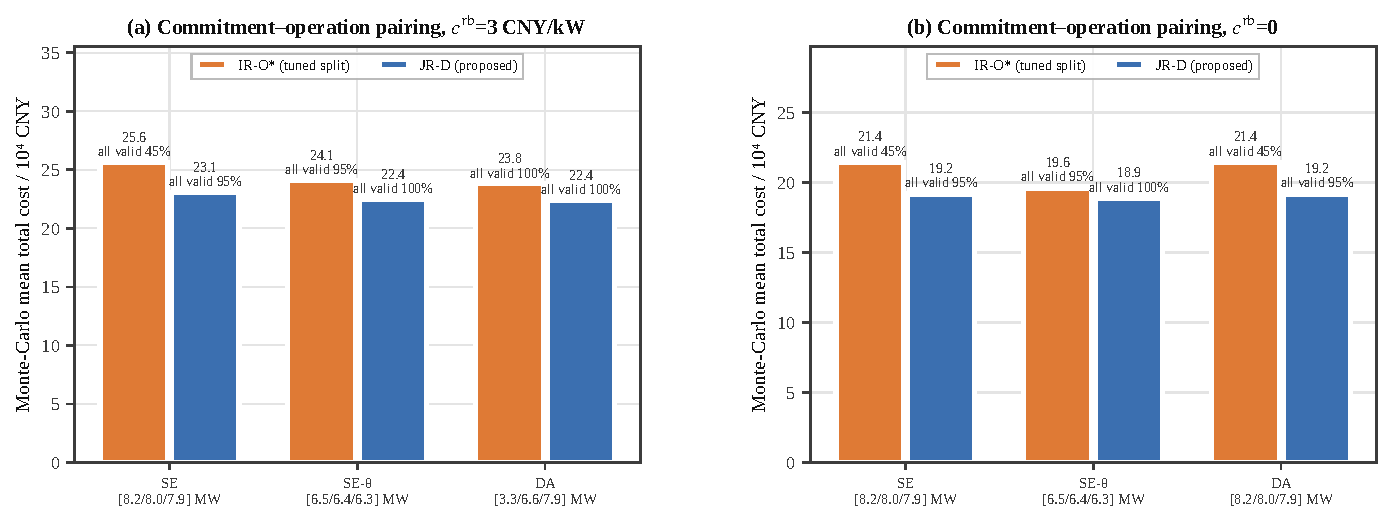
\includegraphics[width=0.86\textwidth]{fig09_commitment.pdf}
\caption{Commitment--operation pairing: mean total cost over 20 operating days with the share of days on which all
three events are valid.}
\label{fig:pairing}
\end{figure*}

The current practice, a single-event assessment operated by independent recovery (SE with IR-O*), keeps all three events
valid on only 45\% of the days. The coupled commitment operated by joint recovery (DA with JR-D) keeps them valid on
every day at a 12.6\% lower cost. Changing only the commitment to DA reduces the cost by 7.2\% (DA with IR-O*), and
operating the DA commitment by JR-D reduces it by a further 5.9\%. In the rebound-priced setting the coupled model
commits less in E1 and keeps the channel for the better-paid E3. In the rule setting the coupled commitment coincides
with the single-event capabilities, and the scaled SE-$\theta$ commitment is better for both operating strategies
because the five day-ahead scenarios cover the high-load tail of the operating days poorly; the risk-averse commitment
below addresses this.

\subsubsection{Risk-averse commitments}
\label{sec:res-risk}

Using ten historical joint scenarios and $\crb=3$, each risk setting of Proposition~\ref{prop:dro} yields a set of
commitments, which JR-D then operates out of sample on the same 52 days (\tabref{tab:risk}, \figref{fig:risk}).

\begin{table}[!t]
\caption{Risk-averse day-ahead commitments evaluated out of sample by JR-D on 52 days.}
\label{tab:risk}
\centering\footnotesize
\setlength{\tabcolsep}{2.8pt}
\begin{tabular}{@{}lcccc@{}}
\toprule
Setting & \makecell{E1/E2/E3 (sum)\\(MW)} & \makecell{Mean\\($10^4$~CNY)} & \makecell{Worst 10\%\\($10^4$~CNY)} & All valid\\
\midrule
SP ($\delta=0$) & 3.66/6.34/7.90 (17.9) & 22.50 & 27.33 & 100\%\\
DRO $\delta=0.2$ & 2.66/6.01/7.90 (16.6) & 22.47 & 27.27 & 100\%\\
DRO $\delta=0.4$ & 2.80/5.06/7.90 (15.8) & 22.45 & 27.24 & 100\%\\
\textbf{DRO $\delta=1.2$} & 0.96/5.77/7.90 (14.6) & \textbf{22.44} & \textbf{27.22} & 100\%\\
RO ($\delta=2$) & 4.54/2.17/7.90 (14.6) & 22.45 & 27.22 & 100\%\\
CVaR$_{0.8}$ & 4.22/2.50/7.90 (14.6) & 22.45 & 27.22 & 100\%\\
Mean--CVaR$_{0.9}$ ($w=0.5$) & 2.74/5.50/7.90 (16.1) & 22.46 & 27.26 & 100\%\\
Single-event assessment & 8.18/7.98/7.90 (24.1) & 23.11 & 29.12 & 96.2\%\\
\bottomrule
\end{tabular}
\end{table}

\begin{figure*}[!t]
\centering
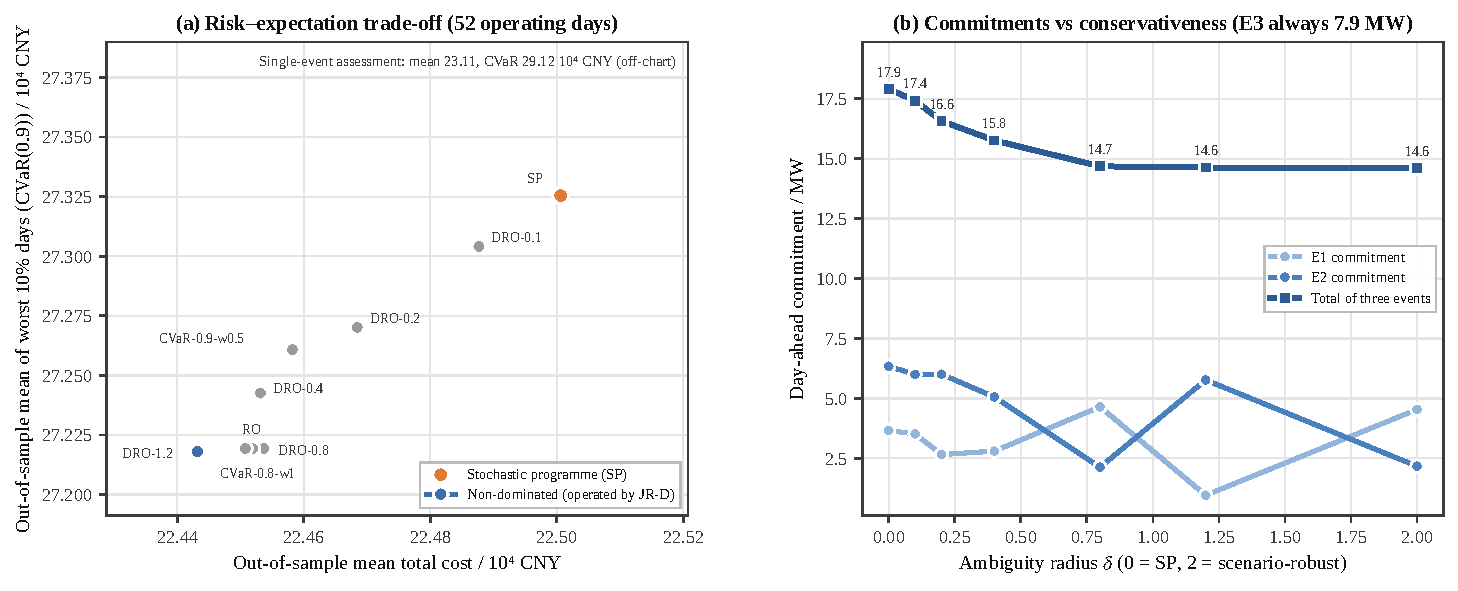
\includegraphics[width=0.86\textwidth]{fig15_risk_pareto.pdf}
\caption{Risk-averse commitments. (a) Out-of-sample mean and mean of the worst 10\% of days for each risk setting on the
52 days (the single-event assessment lies outside the chart); (b) commitments versus the ambiguity radius $\delta$.}
\label{fig:risk}
\end{figure*}

A higher conservativeness lowers the total commitment: as $\delta$ increases from 0 to 0.8, the sum falls monotonically
from 17.9 to 14.7~MW and then stays constant. The best-paid E3 is always committed at its capability of 7.9~MW and the
reduction falls on E1 and E2, between which the model is nearly indifferent, so their split is not unique
(\figref{fig:risk}(b)). The distributionally robust commitments lower both the mean and the tail out of sample: compared
with SP, $\delta$ = 0.4--1.2 reduces the mean by 0.21--0.26\% and the mean of the worst 10\% of days by 0.3--0.4\%, all
paired differences being significant (Wilcoxon $p\le2\times10^{-4}$). $\delta=1.2$ is best in both measures and is the
non-dominated knee point of \figref{fig:risk}(a). The reason is that the ten historical scenarios cover the high-load tail
of the operating days poorly, so SP commits too much and earns less and pays more on adverse days, which the robust
commitments avoid by committing less in E1 and E2. The improvement is small, which shows that coupled commitment with
joint recovery is already robust. Coupled commitments are far better than the single-event assessment, which costs 2.7\%
more on average and 6.6\% more on the worst 10\% of days, with all events valid on only 96.2\% of the days. The DRO
model adds only 21 continuous variables and 30 constraints and solves in 14--25~s with ten scenarios, against 10~s for SP.

\subsubsection{Scenario generation and seasonal drift}
\label{sec:res-scen}

The base commitment uses five equally likely quantile scenarios. Experiment~23 replaces them by K-means scenarios with
non-uniform probabilities ($K$ = 5, 10, 20) and builds a DRO ball with $\delta=0.4$ around them; JR-D then operates each
commitment on the 52 out-of-sample days (\tabref{tab:scen}, \figref{fig:ext}(b)--(d)).

\begin{table}[!t]
\caption{Scenario generation: commitments and costs (52 days, operated by JR-D; costs in $10^4$~CNY).}
\label{tab:scen}
\centering\footnotesize
\setlength{\tabcolsep}{2.4pt}
\begin{tabular}{@{}lccccc@{}}
\toprule
Scenarios & \makecell{E1/E2/E3\\(MW)} & \makecell{In-\\sample} & \makecell{Out-of-\\sample} & \makecell{vs\\quantile-5} & \makecell{In-sample\\underestimate}\\
\midrule
Quantile-5 & 3.27/6.65/7.90 & 19.92 & 22.50 & -- & 13.0\%\\
K-means-5 & 2.42/5.63/7.90 & 20.96 & 22.45 & $-0.19\%$ & 7.1\%\\
K-means-10 & 3.69/4.72/7.90 & 20.68 & 22.46 & $-0.15\%$ & 8.6\%\\
K-means-20 & 3.73/5.51/7.90 & 20.22 & 22.48 & $-0.07\%$ & 11.2\%\\
K-means-5 + DRO & 0.92/6.32/7.90 & 21.10 & 22.45 & $-0.23\%$ & 6.4\%\\
K-means-10 + DRO & 4.71/2.99/7.90 & 20.86 & 22.46 & $-0.19\%$ & 7.6\%\\
\bottomrule
\end{tabular}
\end{table}

\begin{figure*}[!t]
\centering
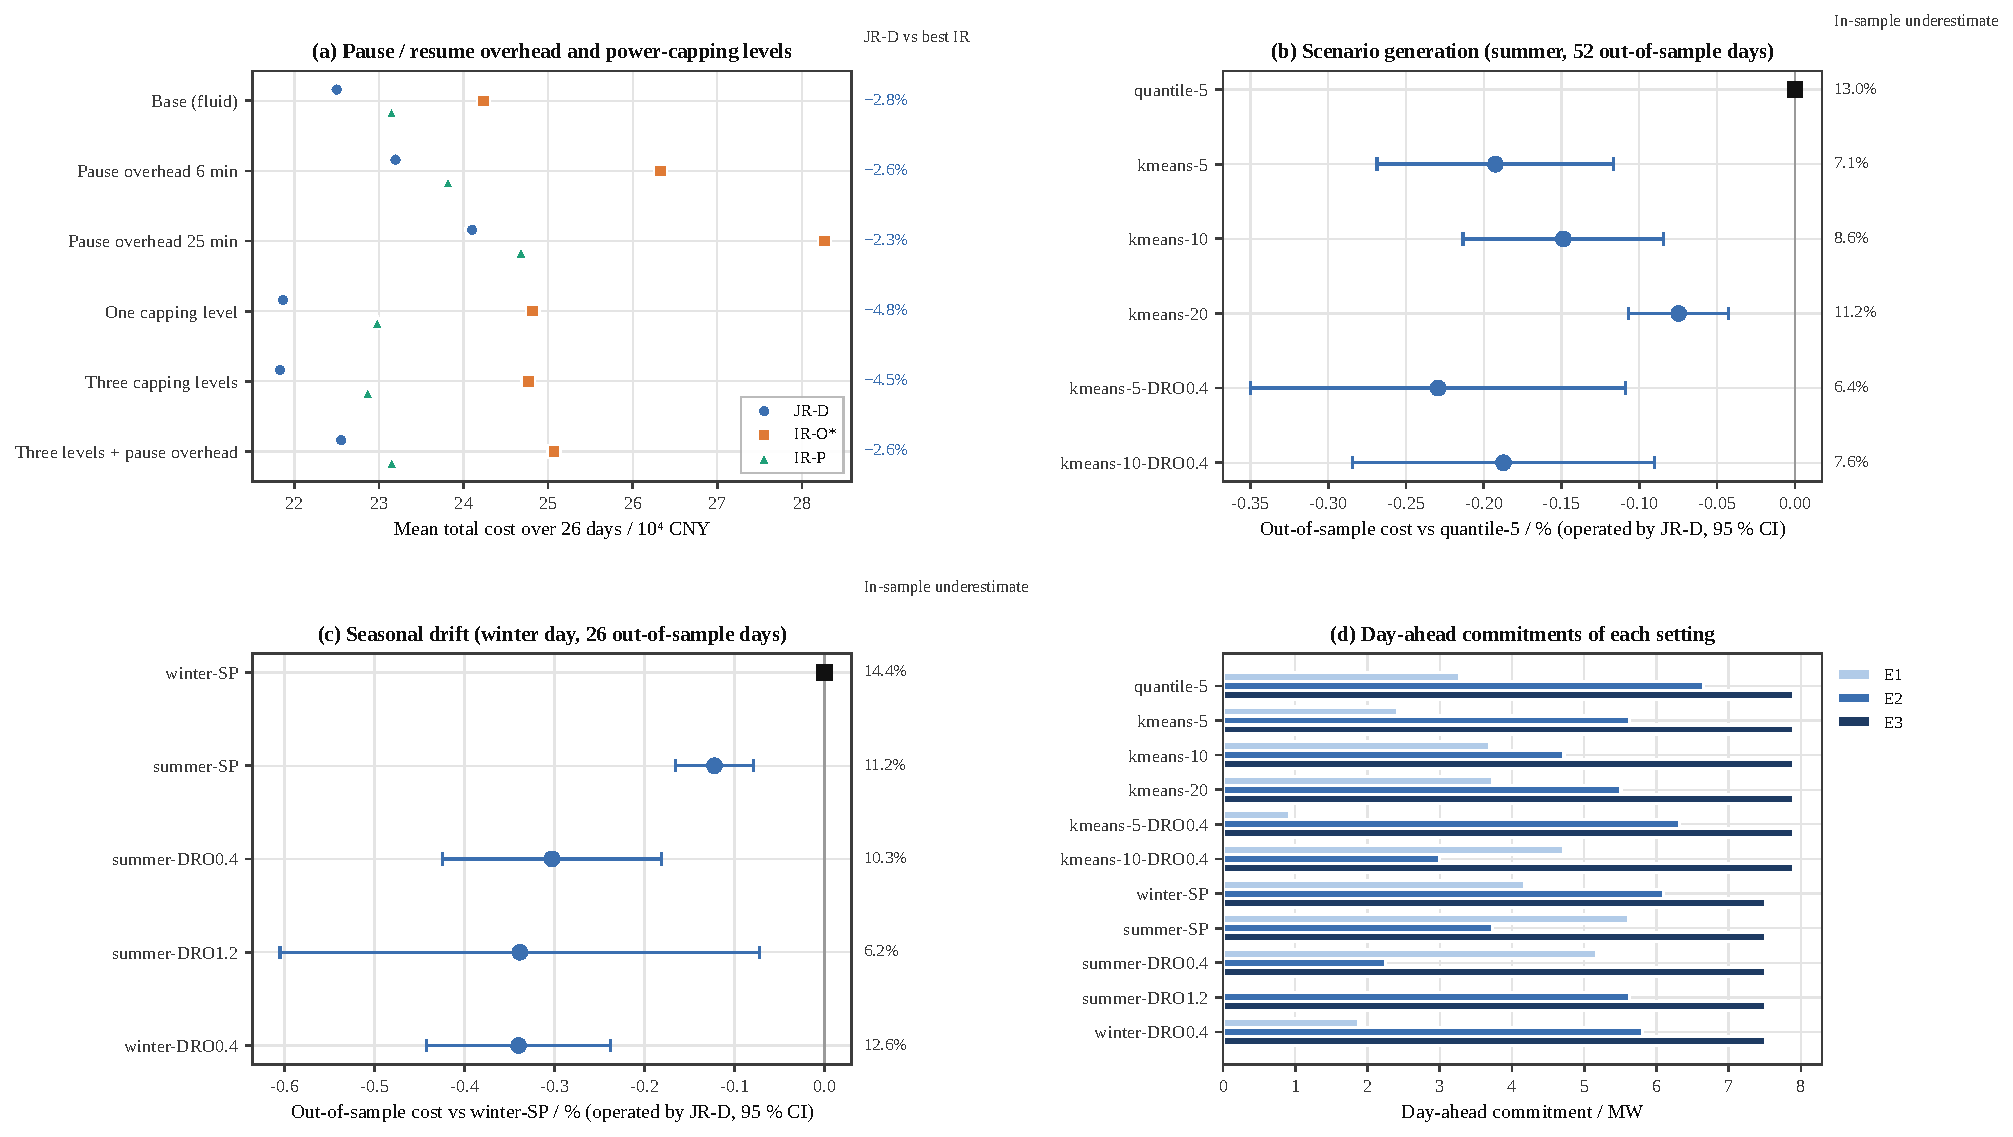
\includegraphics[width=0.96\textwidth]{fig25_extensions.pdf}
\caption{(a) Pause/resume overheads and power-capping levels: mean total cost on 26 operating days (right: JR-D relative
to the strongest independent benchmark); (b)(c) scenario generation and seasonal drift: paired out-of-sample cost
difference to the reference setting (95\% CI; right: underestimate of the in-sample estimate); (d) day-ahead
commitments of each setting.}
\label{fig:ext}
\end{figure*}

The out-of-sample cost is nearly insensitive to scenario generation: the six settings differ by less than 0.23\% and
keep all events valid on every day, although the commitments differ widely (E1 from 0.9 to 4.7~MW, E2 from 3.0 to
6.7~MW). The cost is therefore flat around the optimal commitment, consistent with \secref{sec:res-risk}; the K-means
improvements are statistically significant (Wilcoxon $p\le3\times10^{-5}$) but negligible in size. In-sample estimates
are optimistic by 6--13\%, mainly because the day-ahead model optimises each scenario with perfect information whereas the
operation has only forecasts; K-means-5/10 and DRO reduce the bias to 6--9\%, but 20 scenarios raise it again to 11\%.
Revenue estimates for bidding and investment appraisals should therefore rely on the out-of-sample cost of rolling
operation. A seasonal drift matters little: when the winter case day (10 January 2025) builds its scenarios from the
summer weather pool instead of the winter pool, the commitments change markedly (\figref{fig:ext}(d)) but the cost on 26
out-of-sample winter days is 0.12\% lower rather than higher, with all events valid every day, and DRO with
$\delta$ = 0.4/1.2 lowers it consistently by about 0.3\%.
